% Arquivo principal: configurar o Overleaf para pdfLaTeX + BibTeX.
%\documentclass[a4paper,brazil,ruledheader,normaltoc,capchap]{abnt}

% Para impressão frente e verso (normalização 2011)
\documentclass[a4paper,brazil,ruledheader,normaltoc,capchap,twoside,openany]{abnt_pucmg_utf8}

% Não esquecer das alterações no arquivo abnt.cls
% Se estiver usando o Kile no Ubuntu o arquivo fica armazenado em /usr/share/texmf/tex/latex/abntex.
% Comentar a linha 967 
% \vspace*{30pt}% - Linha comentada para reduzir o espaçamento entre o topo da página e o título \chapter
% Alterar a linha 1143
% \vspace*{-30pt} % - Parâmetro alterado de 30pt para -30pt para reduzir o espaçamento entre o top da página e o título do apêndice
% Alterar a linha 985
%\vspace*{-30pt}\par % - Parâmetro alterado de 0pt para -30pt para reduzir o espaçamento entre o top da página e o título \chapter*
% Alterar a linha 991
% Parâmetro alterado de 45pt para 30pt para reduzir o espaçamento entre o texto e o título \chapter*

% Não esquecer das alterações no arquivo acronym.sty
% Se estiver usando o Kile no Ubuntu o arquivo fica armazenado em /usr/share/texmf-texlive/tex/latex/acronym
% Alterar a linha 225
%\item[\protect\AC@hypertarget{#1}{\acsfont{\normalfont{#2}}} --] #3% - Inserir separador entre acrônimo/descrição e remover o negrito com o normalfont

% Preserva as margens efetivas da versão anterior (o template as redefinia para 1in).
\usepackage[a4paper,margin=1in]{geometry}
% Esta versão local de abntcite detecta hyperref no carregamento.
\usepackage{hyperref}
% Necessário ao ler arquivos .aux antigos produzidos pelo template.
\usepackage[printonlyused]{acronym}

%\usepackage{units}
% Utilize da seguinte forma \unit[78,6]{mA}

% Pacote para citação e referências seguindo ABNT no sistema (AUTOR, Data)
%\usepackage[alf, bibjustif,abnt-emphasize=bf]{abntcite}
\usepackage[alf, abnt-emphasize=em, abnt-thesis-year=title]{abntcite}
% @article An article from a journal or magazine 
% @inproceedings An article in a conference proceedings
% Força que o tipo de ênfase no nome do simpósio seja em caixa alta
\renewcommand{\emph}{\textsc}

% Pacote para múltiplos arquivos .bib
%\usepackage{multibib}
%\newcites{pub}{Refer\^encias das publica\c{c}\~oes}

% Pacote de adequação do formato ABNT para normas da PUCMinas
\usepackage{abnt-PPGInf-PUCMG}

% Pacotes utilitários
\usepackage{graphicx}

% Pacote para fixar a figura no local desejado
\usepackage{float}

\usepackage{url,amsmath}	% Permite melhorias na codificação de fórmulas
\usepackage{xcolor}
% Os gráficos em PDF são gerados localmente dos CSVs: sem pgfplots no Overleaf.
%\usepackage{amsthm}		% Permite melhorias na escrita de teoremas
\usepackage{amssymb}		% Permite utlização de simbolos matemáticos avançados

\usepackage{listings} 		% para importação de código-fonte

\usepackage{setspace}

% Para inserir captions (nova normalização 2011)
\usepackage[size=normalsize,labelfont=bf,textfont={bf},labelsep=endash]{caption}

% Alterar para sequencial a numeração de figuras e tabelas
\captionsetup{figurewithin=none}
\captionsetup{tablewithin=none}

% Para o subsubsection aparecer no sumário 
\setcounter{tocdepth}{3}
\setcounter{secnumdepth}{3}

% Para criar lista de gráficos
\floatstyle{plaintop}
\newfloat{grafico}{H}{loq}
\restylefloat*{grafico}
\floatname{grafico}{Gráfico} 

\renewcommand{\lstlistingname}{Código}
\renewcommand{\lstlistlistingname}{Lista de Códigos}
\citeoption{abnt-etal-cite=1, abnt-and-type=e}

% the bibtex style generates this command, but it's not defined
\newcommand{\optionaltextstyle}{}
% Versão local de abntcite.sty comenta definições usadas nas citações.
\providecommand{\authorcapstyle}{}
\providecommand{\authorstyle}{}
\providecommand{\yearstyle}{}
\providecommand{\citenumstyle}{}

\AtBeginDocument{
  \renewcommand{\thelstlisting}{\arabic{lstlisting}}
}



% PRÉ-TEXTUAIS %%
\begin{document}

\lstset{
  basicstyle=\ttfamily\footnotesize, % Fonte monoespaçada
  numbers=left,                      % Números nas linhas
  numberstyle=\tiny\color{gray},      % Cor dos números
  keywordstyle=\color{blue},          % Palavras-chave em azul
  stringstyle=\color{red},            % Strings em vermelho
  commentstyle=\color{green!50!black},% Comentários em verde-escuro
  morecomment=[l][\color{magenta}]{--}, % Comentários de linha do VHDL (--) em magenta
  backgroundcolor=\color{white},      % Fundo branco
  frame=single,                       % Moldura em volta
  breaklines=true,                    % Quebra linha automática
  captionpos=b,                        % Legenda embaixo
  aboveskip=2em,
  inputencoding=utf8,       % <-- entende acentos
  extendedchars=true,       % <-- entende caracteres estendidos como ç, á, ã
  literate=
    {á}{{\'a}}1 {ã}{{\~a}}1 {â}{{\^a}}1
    {é}{{\'e}}1 {ê}{{\^e}}1
    {í}{{\'i}}1
    {ó}{{\'o}}1 {ô}{{\^o}}1 {õ}{{\~o}}1
    {ú}{{\'u}}1
    {ç}{{\c{c}}}1
    {Á}{{\'A}}1 {Â}{{\^A}}1 {Ã}{{\~A}}1
    {É}{{\'E}}1 {Ê}{{\^E}}1
    {Í}{{\'I}}1
    {Ó}{{\'O}}1 {Ô}{{\^O}}1 {Õ}{{\~O}}1
    {Ú}{{\'U}}1 {Ç}{{\c{C}}}1
}

% Para forçar que elementos pré-textuais (da capa até o sumário) sejam impressos no anverso da folha
\setboolean{@twoside}{false}

\autor{Ian Pereira Pinto Bomfim\\
João Miguel de Abreu Constâncio\\
Ramon Vinícius Silva Corrêa}

% Coloque o título em caixa alta. É o padrão da PUC.
% Vá no arquivo abnt-PPGInf-PUCMG.sty e procure por esse título (linha 575). Altere para o seu título em caixa alta. Isso será utilizado na folha de aprovação.
\titulo{ESTUDO COMPARATIVO DE IMPLEMENTAÇÕES DO QUICKSORT}

%\orientador[Orientador:]{título + nome do orientador}

% Se não tiver, co-orientador, comente a próxima linha.
%\coorientador[Co-orientador:]{Professor}

% Texto
\comentario{Relatório do Trabalho Prático de Projeto e Análise de Algoritmos apresentado à Pontifícia Universidade Católica de Minas Gerais.}

\orientador{Prof. Walisson Ferreira de Carvalho}


% Instituição
\instituicao{Projeto e Análise de Algoritmos \par Pontifícia Universidade Católica de Minas Gerais}

% Local
\local{Belo Horizonte}

% Data
\data{2026}
\capa
%Para forçar que a ficha catalográfica seja impressa no verso da folha de aprovação
\setboolean{@twoside}{true}

% Gera a folha de rosto
\folhaderosto

% Ficha catalográfica
%\include{pre-texto/ficha-catalografica}

% Para forçar que elementos pré-textuais (da capa até o sumário) sejam impressos no anverso da folha
\setboolean{@twoside}{false}

% Folha de aprovação
%\include{pre-texto/folha-aprovacao}

% Dedicatória
%\include{pre-texto/dedicatoria}

% Agradecimentos
%\include{pre-texto/agradecimentos}

% Epígrafe
%\include{pre-texto/epigrafe}

% Resumo
\begin{resumo}
\vspace{-1cm}
\onehalfspacing
Este relatório compara três implementações de Quicksort em Java: recursiva com pivô final, híbrida com Insertion Sort em subvetores pequenos e híbrida com seleção de pivô por mediana-de-três. O limiar $M$ foi calibrado sobre 1.000 valores aleatórios; as versões foram avaliadas com massas aleatórias, crescentes, inversas e com muitos valores repetidos, além de um cenário explícito de pior caso. Para cada configuração houve aquecimento e cinco medições de tempo, comparações e trocas/movimentos. Os resultados registrados selecionaram $M=15$. Em 10.000 valores crescentes, o Quicksort recursivo realizou 49.995.000 comparações, contra 108.986 da versão com mediana-de-três. Em 100.000 valores aleatórios, esta última registrou 11,115 ms contra 14,458 ms da versão recursiva. A escolha da mediana melhora fortemente as entradas ordenadas examinadas, mas não assegura melhora em todas as massas nem elimina o pior caso teórico.
\par\vspace*{.75cm}
\noindent \textbf{Palavras-chave:} Quicksort. Insertion Sort. Mediana-de-três. Análise experimental.
\end{resumo}


% Abstract
% English abstract matching the Portuguese resumo and the recorded experiment.
\begin{abstract}
\vspace{-1cm}
\onehalfspacing
This report compares three Java implementations of Quicksort: a recursive version using the last element as pivot, a hybrid version using Insertion Sort on small subarrays, and a hybrid version using median-of-three pivot selection. The cutoff threshold $M$ was calibrated on 1,000 random values. The implementations were evaluated on random, ascending, descending, and duplicate-rich arrays, as well as an explicit worst-case scenario for the last-element pivot. Each configuration included warm-up runs and five measured executions, recording elapsed time, value comparisons, and swaps/movements. The recorded calibration selected $M=15$. On 10,000 ascending values, recursive Quicksort performed 49,995,000 comparisons, compared with 108,986 for the median-of-three version. On 100,000 random values, the latter took 11.115 ms, compared with 14.458 ms for the recursive version. Median-of-three selection substantially improved performance on the ordered inputs examined, but it neither outperformed the other versions on every input nor eliminated the theoretical worst case.
\par\vspace*{.75cm}
\noindent \textbf{Keywords:} Quicksort. Insertion Sort. Median-of-three. Experimental analysis.
\end{abstract}


\makeatletter
\renewcommand\numberline[1]{
	\leftskip 0em
	\rightskip 1.6em
	\parfillskip -\rightskip
	\parindent 0em
	\@tempdima 2.0em
	\vspace{0em} \advance\leftskip \@tempdima \null\nobreak\hskip -\leftskip
	FIGURA \normalfont #1 -- }
\makeatother

% Sem figuras neste relatório (os gráficos têm ambiente próprio).
%\listoffigures

\makeatletter
\renewcommand\numberline[1]{
	\leftskip 0em
	\rightskip 1.6em
	\parfillskip -\rightskip
	\parindent 0em
	\@tempdima 2.0em
	\vspace{0em} \advance\leftskip \@tempdima \null\nobreak\hskip -\leftskip
	TABELA \normalfont #1 -- }
\makeatother

% Lista de tabelas
\listoftables

\makeatletter
\renewcommand\numberline[1]{
	\leftskip 0em
	\rightskip 1.6em
	\parfillskip -\rightskip
	\parindent 0em
	\@tempdima 2.0em
	\vspace{0.5em} \advance\leftskip \@tempdima \null\nobreak\hskip -\leftskip
	GRÁFICO \normalfont #1 -- }
\makeatother

% Lista dos gráficos comparativos por cenário
\listof{grafico}{Lista de Gráficos}

% Lista de siglas
%% Lista de Abreviaturas e Siglas
%\chapter*{Lista de Abreviaturas e Siglas}
\chapter*{Lista de Abreviaturas e Siglas}

% Mantenha sempre em ordem alfabética.

\begin{acronym}
\acro{BER} {\textit{Bit Error Rate}}
\acro{BT} {\textit{Block Tri-diagonal}}
\acro{CG} {\textit{Conjugate Gradient}}
\acro{CSS} {\textit{Chirp Spread Spectrum}}
\acro{DCC-MAC} {\textit{Dynamic Channel Coding} MAC}
\acro{DSSS} {\textit{Direct-sequence spread spectrum}}
\acro{EP} {\textit{Embarrassingly Parallel}}
\acro{FIFO} {\textit{First In, First Out}}
\acro{FT} {\textit{Fast Fourier Transform}}
\acro{IEEE} {\textit{Institute of Electrical and Electronics Engineers}}
\acro{IR-UWB} {\textit{Impulse Radio} UWB}
\acro{IS} {\textit{Integer Sort}}
\acro{LU} {\textit{Lower-Upper Gauss-Seidel}}
\acro{MAC} {\textit{Medium Access Control}}
\acro{MB-OFDM} {\textit{Multi-Band Orthogonal Frequency Division Multiplexing}}
\acro{MG} {\textit{Multi-Grid}}
\acro{MPE} {MPI \textit{Parallel Environment}}
\acro{MPI} {Interface de passagem de mensagem, do inglês \textit{Message Passing Interface}}
\acro{NAS} {NASA \textit{Advanced Supercomputing}}
\acro{NOAH} {\textit{No Ad-Hoc Routing Agent}} 
\acro{NS-2} {\textit{Network Simulator} 2}
\acro{NoCs} {Redes-em-Chip, do inglês \textit{Networks-on-Chip}}
\acro{NPB} {NAS \textit{Parallel Benchmark}}
\acro{OpenMP} {Multi-processamento aberto, do inglês \textit{Open Multi-Processing}}
\acro{PHY} {\textit{Physical Layer}}
\acro{PPM} {\textit{Pulse-Position Modulation}}
\acro{SP} {\textit{Scalar Penta-diagonal}}
\acro{TH} {\textit{Time Hopping}}
\acro{THS} {\textit{Time Hopping Sequence}}
\acro{UDP}{\textit{User Datagram Protocol}}
\acro{UWB} {\textit{Ultra Wide Band}}
\acro{WiNoCs} {Redes-em-Chip Sem Fio, do inglês \textit{Wireless Networks-on-Chip}}
\acro{WLAN} {Rede Local Sem Fio, do inglês \textit{Wireless Local Area Network}}
\acro{WPAN} {Rede de Área Pessoal Sem Fio, do inglês \textit{Wireless Personal Area Network}}
\end{acronym}

\makeatletter
\renewcommand\numberline[1]{#1\hspace{0.8em}}
\makeatother

% Altera para espaçamento simples a partir daqui
\singlespacing

% Sumário
\tableofcontents

% Altera para espaçamento 1,5 a partir daqui
\onehalfspacing

%% TEXTUAIS 
% Para forçar que elementos textuais e pós-textuais sejam impressos no anverso e verso das folhas
\setboolean{@twoside}{true}
% Altere o número da página para o correto. Conte todas as páginas frente e verso, menos a capa, nclusive a ficha catalográfica até a página do primeiro capítulo.
\setcounter{page}{1}

% Capítulos
% Para forçar que o capítulo de introdução comece no anverso
\setboolean{@openright}{true}
\chapter{Introdução}
\label{intro}

A ordenação de dados é uma etapa recorrente em buscas, processamento de registros e preparação de informações para outros algoritmos. O Quicksort combina partições sucessivas e execução rápida em muitas entradas, mas sua eficiência depende da escolha do pivô e da distribuição dos valores. Em particular, uma implementação que escolhe sempre o último elemento pode sofrer degradação quadrática em vetores já ordenados \cite{cormen2012,gfg_quick}.

Este trabalho investiga como duas alterações práticas afetam essa implementação: interromper a recursão em subvetores pequenos e ordená-los por inserção; e escolher o pivô pela mediana do primeiro, do elemento central e do último. O objetivo é comparar o Quicksort recursivo, o híbrido e o híbrido com mediana-de-três em tempo médio, comparações de valores e trocas/movimentos, usando massas idênticas de dados aleatórios, crescentes, decrescentes e com duplicatas. Um cenário crescente identifica explicitamente o pior caso da escolha do pivô final.

As perguntas que orientam a comparação são: em quais entradas interromper a partição melhora o tempo sem alterar a estratégia de pivô; em quais entradas a mediana-de-três evita a degradação observada com pivô final; e até que ponto as contagens de operações ajudam a explicar diferenças de tempo? O estudo distingue uma melhora \emph{observada} numa execução de uma garantia de complexidade para todas as entradas. Seu escopo é a implementação instrumentada em Java e as massas efetivamente geradas, não uma comparação de bibliotecas de ordenação nem uma prova de superioridade universal.

O Capítulo~\ref{cap:desenvolvimento} apresenta o referencial teórico; o Capítulo~\ref{cap:metodologia} detalha o protocolo de medição. O Capítulo~\ref{cap:algoritmos} analisa os algoritmos e suas condições de custo; o Capítulo~\ref{cap:resultados} apresenta os dados exportados pelo projeto e sua interpretação. O Capítulo~\ref{cap:conclusao} sintetiza as conclusões e limitações.

% Os demais capítulos não precisam começar no anverso
\setboolean{@openright}{false}
\chapter{Referencial teórico}
\label{cap:desenvolvimento}

\section{Ordenação por inserção}

O Insertion Sort percorre um vetor da esquerda para a direita, deslocando valores maiores que a chave corrente até abrir espaço para sua inserção. É estável em sua forma usual e pode operar com espaço auxiliar constante. Com $n$ elementos em ordem crescente, cada chave exige apenas uma comparação relevante e o trabalho é $\Theta(n)$; em ordem inversa, os deslocamentos somam $\sum_{i=1}^{n-1}i=n(n-1)/2$, produzindo $\Theta(n^2)$ em tempo e comparações. Em vetores pequenos, entretanto, o laço simples e a baixa sobrecarga justificam seu emprego como caso-base de algoritmos híbridos \cite{gfg_insertion,gfg_insertion_complexity}.

Por exemplo, ao inserir sucessivamente as chaves de $[5,2,4,1]$, os prefixos ordenados passam por $[2,5,4,1]$, $[2,4,5,1]$ e $[1,2,4,5]$. A chave $1$ desloca três predecessores; na convenção adotada no código, isso representa três deslocamentos e uma inserção final, não quatro trocas entre pares. O prefixo só é alterado quando há um predecessor estritamente maior: elementos iguais não são deslocados pela inserção. A ordenação por inserção isolada tem custo médio quadrático sob permutações aleatórias de chaves distintas e, no melhor caso, usa $n-1$ comparações entre valores.

\section{Quicksort e seleção do pivô}

O Quicksort escolhe um pivô, particiona os demais valores em torno dele e ordena recursivamente as duas regiões. Para uma partição linear, a recorrência é $T(n)=T(k)+T(n-k-1)+\Theta(n)$. Partições próximas da metade dão $\Theta(n\log n)$; partições com uma região vazia dão $T(n)=T(n-1)+\Theta(n)=\Theta(n^2)$. Para entradas aleatórias sob hipóteses usuais de distribuição, o número esperado de operações é $\Theta(n\log n)$. A pilha recursiva requer $O(\log n)$ espaço em partições equilibradas e pode alcançar $O(n)$ em partições degeneradas \cite{cormen2012,gfg_quick}.

Neste trabalho, a partição de Lomuto usa o último valor como pivô e encaminha valores menores \emph{ou iguais} para a esquerda. Assim, uma entrada crescente com valores distintos põe sempre o maior valor no fim: as comparações são exatamente $\sum_{i=1}^{n-1}i=n(n-1)/2$. Na entrada decrescente, o pivô alterna entre extremos, ainda produzindo partições desbalanceadas. Elementos todos iguais também se concentram à esquerda, revelando uma limitação da partição em duas vias.

Uma partição concreta esclarece a diferença entre ordenar o vetor e posicionar apenas o pivô. Em $[4,1,3,2]$, o pivô final é $2$: a varredura encontra $1\leq2$, coloca-o à esquerda e, ao final, posiciona $2$ após $1$. O vetor resultante dessa partição é $[1,2,3,4]$ neste exemplo particular; em geral, as duas regiões ainda precisam das chamadas recursivas. Foram realizadas três comparações com o pivô nessa partição. Para $[1,2,3,4]$, por outro lado, o pivô $4$ já está no extremo correto; a primeira partição deixa uma região de três elementos e outra vazia, repetindo o desbalanceamento até chegar a um elemento.

\section{Hibridização e escolha do pivô}

Substituir por Insertion Sort a recursão em partições de tamanho menor que $M$ reduz a sobrecarga para pequenos segmentos, mas não altera o pivô das partições grandes. Por isso, isoladamente, a hibridização não remove o pior caso $\Theta(n^2)$. A mediana-de-três escolhe o valor intermediário entre as posições inicial, central e final; tende a evitar pivôs extremos em dados crescentes ou decrescentes, mas tampouco garante partições equilibradas para toda entrada, em especial quando há muitos valores iguais. O emprego de Insertion Sort em segmentos pequenos e o impacto da escolha do pivô são discutidos em \cite{gfg_insertion,gfg_quick}; a limitação com chaves iguais decorre da partição usada neste projeto.

Na implementação estudada, os candidatos são \emph{valores} das posições primeira, central e última, e não a média aritmética deles. Em $[9,4,5,7,1]$, por exemplo, a mediana dos candidatos $9$, $5$ e $1$ é $5$; depois de rearranjá-los, o código leva essa mediana à posição final para reutilizar a mesma partição. Trata-se de uma ilustração da escolha do pivô: com o $M=15$ medido neste estudo, um vetor de apenas cinco elementos seria ordenado diretamente por Insertion Sort, sem executar a seleção por mediana. A comparação real entre H e M3 mantém o mesmo limiar; diferenças entre essas versões decorrem da estratégia de pivô nas partições que chegam a ser executadas.

O livro de \citeonline{ziviani2011} apresenta métodos clássicos de ordenação, entre eles a inserção e o Quicksort. Para o esquema concreto examinado aqui, \citeonline{gfg_quick} descreve a partição de Lomuto com pivô final e a degradação quando as partições são desequilibradas. A condição $\leq$ do código apresentado no Capítulo~\ref{cap:algoritmos} também encaminha valores iguais ao pivô para um mesmo lado. Essas observações motivam as duas mudanças avaliadas neste trabalho, mas não asseguram pior caso $O(n\log n)$ para a implementação estudada.

\begin{table}[htbp]
\centering
\caption{Custos assintóticos esperados e limites relevantes para este estudo}
\label{tab:complexidades}
\begin{tabular}{l c c c}
\hline
Algoritmo & Melhor caso & Caso médio usual & Pior caso \\
\hline
Insertion Sort (isolado) & $\Theta(n)$ & $\Theta(n^2)$ & $\Theta(n^2)$ \\
Quicksort recursivo & $\Theta(n\log n)$ & $\Theta(n\log n)$ & $\Theta(n^2)$ \\
Híbrido, $M$ constante & $\Theta(n\log n)$ & $\Theta(n\log n)$ & $\Theta(n^2)$ \\
Híbrido com mediana, $M$ constante & $\Theta(n\log n)$ & $\Theta(n\log n)$ & $\Theta(n^2)$ \\
\hline
\end{tabular}
\par\smallskip\footnotesize Fonte: análise do código; caso médio sob condições usuais de entradas aleatórias.\normalsize
\end{table}

Para as três versões de Quicksort, a partição ocupa espaço auxiliar constante, mas a API clona o vetor ($\Theta(n)$ de espaço) e a pilha recursiva pode chegar a $\Theta(n)$ em partições degeneradas. Na forma equilibrada, a pilha requer $\Theta(\log n)$. As ordens da tabela descrevem o crescimento com $n$ e $M$ fixo: uma redução em comparações numa massa específica não muda, por si só, o limite de pior caso do algoritmo.

\chapter{Metodologia}
\label{cap:metodologia}

\section{Implementação e massas de teste}

O código estudado foi implementado em Java 17, no projeto \texttt{tp-1-paa-quicksort}. As três versões retornam um clone do vetor de entrada. A versão recursiva e a híbrida usam partição de Lomuto com pivô no último índice; a versão melhorada ordena os três candidatos (primeiro, meio e último), move a mediana para o fim e usa a mesma partição. Nas versões híbridas, segmentos com \emph{menos} de $M$ elementos são ordenados diretamente por Insertion Sort. O mesmo $M$ é usado nas duas versões, de modo que apenas a seleção do pivô muda entre elas.

O gerador pseudoaleatório Java usa semente 42. Para a massa aleatória, sorteia inteiros em $[0,10n)$; para muitos duplicados, em $[0,\max(1,\lfloor n/10\rfloor))$. Vetores crescentes contêm $0,1,\ldots,n-1$ e os inversos contêm essa sequência revertida. O cenário denominado \emph{pior caso} repete exatamente a massa crescente, mas identifica explicitamente o efeito do pivô final inadequado. O estado do gerador é avançado ao longo dos cenários e tamanhos; a semente permite reproduzir a sequência ao executar o estudo completo.

As massas aleatória e com muitos duplicados têm nove tamanhos: 100, 500, 1.000, 2.000, 5.000, 10.000, 20.000, 50.000 e 100.000. As massas crescente, inversa e de pior caso têm seis: 100, 500, 1.000, 2.000, 5.000 e 10.000. O pior caso inclui ainda $n=200$. Os cenários degenerados são limitados a 10.000 para reduzir custo quadrático e risco de esgotamento da pilha. São 37 combinações de massa/tamanho e três versões, totalizando 111 linhas de resultados.

\begin{table}[htbp]
\centering
\caption{Planejamento das massas e objetivo de cada cenário}
\label{tab:massas}
\begin{tabular}{p{3cm} p{7cm} r}
\hline
Cenário & Propriedade examinada & Tamanhos \\
\hline
Aleatório & Pivôs e posições sem ordenação inicial; valores em $[0,10n)$ & 9 \\
Crescente & Pivô final máximo; partição degenerada com chaves distintas & 6 \\
Decrescente & Pivô final alternando extremos após as partições & 6 \\
Duplicados & Repetição de chaves com até $\max(1,\lfloor n/10\rfloor)$ valores possíveis & 9 \\
Pior caso & Nova medição da massa crescente, para evidenciar o pivô final & 7 \\
\hline
\end{tabular}
\par\smallskip\footnotesize Fonte: \texttt{TestDataGenerator.java} e \texttt{QuickSortComparativeStudy.java}.\normalsize
\end{table}

No gerador de duplicados, o número de valores possíveis aumenta com $n$. Portanto, ``muitos duplicados'' não significa que uma fração fixa de 90\% das posições contenha o mesmo valor, nem que todas as chaves sejam iguais. Os cenários crescente e pior caso têm entradas iguais para o mesmo tamanho, mas são medições separadas e seus tempos não precisam coincidir. Assim, a repetição do cenário não constitui uma segunda construção adversa independente para M3.

\section{Calibração, medições e validação}

Antes da comparação, o híbrido com pivô final é avaliado com dez candidatos a $M$: 5, 10, 15, 20, 25, 30, 40, 50, 75 e 100. Usa-se um único vetor aleatório de 1.000 elementos, semente 42: cinco aquecimentos e dez medições por candidato, escolhendo-se o menor tempo médio. A calibração não utiliza a versão com mediana-de-três nem as outras distribuições, de modo que o valor encontrado é específico da massa e da execução registrada.

O procedimento de seleção compara os dez candidatos sobre \emph{cópias dos mesmos valores}; variar $M$ não altera a massa de calibração. O limiar de corte é estrito: segmentos de tamanho $M-1$ seguem para Insertion Sort, enquanto os de tamanho $M$ ainda são particionados. Fixar $M$ para H e M3 permite atribuir diferenças de comportamento à escolha do pivô, sem introduzir um limiar distinto como segunda variável experimental. Os dez tempos de calibração são médias de execuções cronometradas, não dez valores alternativos de $M$ extraídos de execuções diferentes do estudo completo.

Em cada cenário/tamanho, as três versões recebem cópias dos mesmos valores. Cada versão passa por três aquecimentos e cinco execuções medidas. \texttt{System.nanoTime()} envolve somente a chamada ao método de ordenação: inclui o clone interno produzido por ele, mas exclui a cópia de entrada preparada pelo medidor, geração de dados, validação e escrita de arquivos. Os resultados são confrontados com \texttt{Arrays.sort}, que ordena vetores de inteiros em ordem crescente \cite{oracle2021}. As médias registradas para tempo e contadores são divisões inteiras das somas pelas cinco execuções; os tempos no CSV são nanossegundos, convertidos aqui para milissegundos ($1\,\mathrm{ms}=10^6\,\mathrm{ns}$).

O contador de comparações inclui somente comparações entre valores, inclusive as três verificações por escolha de mediana, e não condições de laço. O contador de \emph{trocas/movimentos} inclui trocas entre índices distintos no Quicksort e deslocamentos mais inserção final no Insertion Sort; essas quantidades não representam a mesma operação física. Os dados foram transcritos dos arquivos \path{arrays_testados/calibracao_m.csv} e \path{arrays_testados/resultados.csv}. Sem o registro da carga da máquina durante os testes não se atribui significância estatística às pequenas diferenças de tempo nem se generaliza a outra plataforma.

O intervalo entre duas chamadas a \texttt{System.nanoTime()} fornece duração transcorrida em nanossegundos, não uma data/hora nem tempo de CPU isolado \cite{oracle2021}. O aquecimento pode reduzir interferências de carregamento e compilação dinâmica, mas não elimina coleta de lixo, interferência de outros processos ou efeitos de cache. O projeto armazena apenas a média inteira das cinco medições, não os cinco tempos individuais nem uma estimativa de dispersão. Por isso, uma diferença pequena entre médias não autoriza afirmar que uma versão é estatisticamente mais rápida; comparações exatas de operações nas entradas determinísticas constituem evidência de natureza diferente da flutuação do tempo.

\section{Procedimento e organização dos arquivos}

O estudo é aplicado e comparativo, não uma simulação assintótica: os contadores descrevem a execução do código instrumentado e o cronômetro mede o tempo de parede decorrido na chamada de ordenação, \emph{não} tempo de CPU isolado. O fluxo executado foi: (1) calibrar $M$ no híbrido de pivô final; (2) gerar cada massa com semente fixa; (3) armazenar seu vetor original; (4) aquecer separadamente cada implementação; (5) executar cinco ordenações de cópias equivalentes; (6) confrontar cada saída com \texttt{Arrays.sort}; (7) calcular médias inteiras e exportar os vetores ordenados e as estatísticas. As versões são medidas sequencialmente, não em ordem aleatorizada; por isso os efeitos de aquecimento residual, coleta de lixo e carga do sistema não são controlados completamente.

Dentro de \path{arrays_testados/}, cada cenário guarda entradas originais, saídas ordenadas e resumos em três subpastas próprias. A calibração está em \path{arrays_testados/calibracao_m.csv} e as 111 médias em \path{arrays_testados/resultados.csv}, com ponto e vírgula separando campos. O arquivo \path{texto/resultados_detalhados.tex} deste relatório foi gerado diretamente desse CSV pelo script \path{gerar_dados_relatorio.js}, após verificar o número de linhas, a coluna de sucesso e $M=15$. Assim, tabelas e gráficos podem ser conferidos com o mesmo registro, sem copiar números do documento de referência.

O código-fonte e os testes estão disponíveis no repositório do projeto: \url{https://github.com/ramonVSCorrea/tp-1-paa-quicksort}. Os arquivos de \path{arrays_testados/} são gerados pela execução; os resultados registrados neste relatório correspondem aos CSVs da execução analisada.

\section{Ambiente de execução}

Os testes foram executados em um equipamento com a seguinte configuração:

\begin{itemize}
  \item Processador Intel Core i5-9300H, frequência nominal de 2,40\,GHz;
  \item 16,0\,GB de memória RAM instalada (15,8\,GB utilizáveis);
  \item Windows 11 Education, versão 26H2, compilação 26300.9550, em sistema operacional de 64 bits e processador x64;
  \item Java Temurin OpenJDK 17.0.20.1 (64 bits; build 17.0.20.1+1).
\end{itemize}

\chapter{Análise das implementações}
\label{cap:algoritmos}

Esta análise associa o custo teórico às condições e aos contadores do \emph{código efetivamente executado}. Os trechos seguintes são recortes representativos das classes Java do projeto; nomes e testes preservam a lógica original. Em todas as versões, o método público retorna uma cópia do vetor, custo adicional $\Theta(n)$ de tempo e espaço, já incluído no relógio. A partição propriamente dita é local ao clone; logo, não se deve confundir espaço auxiliar da partição ($O(1)$) com espaço total desta API ($O(n)$ mais a pilha).

\section{Insertion Sort para subvetores pequenos}

O algoritmo mantém o prefixo anterior à posição atual ordenado. Para cada chave, desloca os predecessores estritamente maiores; a comparação estrita preserva a ordem relativa entre iguais. O Código~\ref{cod:insercao} destaca a contagem exata usada no projeto: a comparação entre valores ocorre a cada iteração interna não interrompida pelo limite esquerdo; só há incremento do contador de movimentos se há deslocamento ou inserção em índice diferente.

\begin{lstlisting}[language=Java,caption={Operações centrais de InsertionSort.java},label={cod:insercao}]
for (int currentIndex = low + 1; currentIndex <= high; currentIndex++) {
    int valueToInsert = array[currentIndex];
    int comparisonIndex = currentIndex - 1;
    while (comparisonIndex >= low) {
        metrics.incrementComparisons();
        if (array[comparisonIndex] > valueToInsert) {
            array[comparisonIndex + 1] = array[comparisonIndex];
            metrics.incrementSwaps(); // deslocamento, nao troca
            comparisonIndex--;
        } else break;
    }
    if (comparisonIndex + 1 != currentIndex) {
        array[comparisonIndex + 1] = valueToInsert;
        metrics.incrementSwaps(); // insercao final
    }
}
\end{lstlisting}

Se $s_i$ for o número de predecessores maiores deslocados ao inserir a $i$-ésima chave, o contador de movimentos cresce em $s_i+\mathbf{1}_{s_i>0}$. O número de comparações entre valores é $s_i+1$ se houver um predecessor final não deslocado, ou $s_i$ quando o início do segmento é alcançado. Para um subvetor de $m$ elementos crescente, são $m-1$ comparações e zero movimentos contados; para o inverso, há $m(m-1)/2$ comparações e $m(m-1)/2+(m-1)$ movimentos. Essas contagens decorrem da instrumentação mostrada no Código~\ref{cod:insercao}; o custo médio e o pior caso do Insertion Sort para um subvetor arbitrário são $\Theta(m^2)$ \cite{cormen2012}.

Em uma permutação uniforme de $m$ chaves distintas, cada par está invertido com probabilidade $1/2$; pela linearidade da esperança, o número esperado de deslocamentos da inserção é $m(m-1)/4$ \cite{gfg_insertion_complexity}. Os testes finais que interrompem o laço e as inserções após deslocamentos acrescentam no máximo $O(m)$ operações. Essa dedução explica a ordem média quadrática sem equiparar o número de deslocamentos ao de trocas de posições do Quicksort. Quando o algoritmo atua apenas sobre blocos de comprimento inferior a $M$, a mesma análise vale em cada bloco, não automaticamente para o vetor inteiro como se ele fosse ordenado apenas por inserção.

\section{Quicksort recursivo com pivô final}

A partição do Código~\ref{cod:particao} compara cada um dos $m-1$ elementos não pivôs com o valor final. O índice de partição avança somente quando a condição $\leq$ é satisfeita. Trocas com índices idênticos são ignoradas, inclusive a troca final se o pivô já estiver na posição correta. Após colocar o pivô, são realizadas chamadas nos intervalos estritamente à esquerda e à direita de sua posição definitiva.

\begin{lstlisting}[language=Java,caption={Partição usada por RecursiveQuickSort.java e HybridQuickSort.java},label={cod:particao}]
int pivotValue = array[high];
int partitionIndex = low - 1;
for (int currentIndex = low; currentIndex < high; currentIndex++) {
    metrics.incrementComparisons();
    if (array[currentIndex] <= pivotValue) {
        partitionIndex++;
        swap(array, partitionIndex, currentIndex, metrics);
    }
}
swap(array, partitionIndex + 1, high, metrics);
return partitionIndex + 1;
\end{lstlisting}

Para uma partição em $k$ elementos à esquerda, a recorrência dos custos de ordenação é
\begin{equation}
 T(n)=T(k)+T(n-k-1)+a(n-1)+b,\qquad T(0),T(1)=\Theta(1),
 \label{eq:quick}
\end{equation}
para constantes $a,b>0$. No melhor padrão de partições, $k\simeq(n-1)/2$, obtém-se $\Theta(n\log n)$. Sob uma permutação aleatória de chaves distintas e pivô fixo no fim, a posição do pivô é uniforme entre as posições possíveis; portanto o número esperado de comparações também é $\Theta(n\log n)$ \cite{cormen2012}. Já quando $k=0$ ou $k=n-1$ repetidamente, a contagem do código é exata:
\begin{equation}
 C_{\mathrm{R}}(n)=\sum_{m=2}^{n}(m-1)=\frac{n(n-1)}{2}=\Theta(n^2).
 \label{eq:quadratico}
\end{equation}
É precisamente o que ocorre na massa crescente de chaves distintas, e também no inverso com esta partição. Na crescente, os testes são verdadeiros mas as posições trocadas são idênticas; isso justifica simultaneamente milhões de comparações e zero trocas efetivas. A versão recursiva não elimina recursão de cauda nem impõe profundidade máxima: sua pilha alcança $\Theta(n)$ nessas entradas.

Para uma permutação uniforme de $n$ chaves \emph{distintas}, cada posição final possível do pivô é igualmente provável. Se $E[C(n)]$ é a esperança de comparações entre valores na versão recursiva, a partição de Lomuto e a distribuição uniforme das subpermutações dão
\begin{equation}
 E[C(n)]=n-1+\frac{2}{n}\sum_{k=0}^{n-1}E[C(k)],\qquad E[C(0)]=E[C(1)]=0.
 \label{eq:medioquick}
\end{equation}
Resolvendo a Equação~\ref{eq:medioquick}, obtém-se $E[C(n)]=2(n+1)H_n-4n$, com $H_n=\sum_{i=1}^{n}1/i$, que cresce como $\Theta(n\log n)$. Essa expressão exata é deduzida da recorrência acima, enquanto a análise do crescimento esperado do Quicksort é discutida por \citeonline{cormen2012}. A fórmula não descreve literalmente o gerador de aleatórios do experimento, que admite valores repetidos, nem a mediana-de-três, cujo pivô não tem a mesma distribuição uniforme. Ela serve de referência teórica para interpretar a escala observada sem ajustar uma lei exata aos pontos do CSV.

\section{Quicksort híbrido e efeito do limiar}

O Código~\ref{cod:corte} mostra a condição \texttt{subarraySize < threshold}, que envia segmentos de até $M-1$ elementos à inserção. Portanto, \textbf{tamanho igual a $M$ ainda é particionado}, ao contrário de variantes que usam $\leq M$. O teste só é alcançado em segmentos com ao menos dois elementos. Com $M=15$ e a massa crescente, a recursão vai de $n$ até 15, seguida pela inserção de um bloco crescente de 14 elementos. Em particular, o total de comparações H é
\begin{equation}
 C_{\mathrm{H}}(n)=\sum_{m=15}^{n}(m-1)+13
 =\frac{n(n-1)}{2}-78,\quad n\geq15.
 \label{eq:hibridocrescente}
\end{equation}
Para $n=10.000$, a equação fornece 49.994.922, exatamente o CSV. Quando as partições são aproximadamente equilibradas, há $O(\log(n/M))$ níveis. A soma das partições custa $O(n\log(n/M))$; os blocos finais de menos de $M$ elementos custam, em agregado, $O(nM)$ no pior caso local. Com $M$ constante, a ordem usual segue $O(n\log n)$, mas partições repetidamente degeneradas mantêm $\Theta(n^2)$. A fórmula por níveis não deve ser aplicada ao caso degenerado como se os blocos fossem equilibrados.

\begin{lstlisting}[language=Java,caption={Condição de corte em HybridQuickSort.java},label={cod:corte}]
int subarraySize = high - low + 1;
if (subarraySize < threshold) {
    InsertionSort.sort(array, low, high, metrics);
} else {
    int pivotIndex = partition(array, low, high, metrics);
    quickSort(array, low, pivotIndex - 1, metrics);
    quickSort(array, pivotIndex + 1, high, metrics);
}
\end{lstlisting}

\section{Quicksort híbrido com mediana-de-três}

O Código~\ref{cod:mediana} mostra a seleção real: comparam-se primeiro e meio, meio e último, primeiro e meio outra vez, rearranjando os três candidatos quando necessário. O índice central contém então o valor mediano, que é movido para o fim antes da mesma partição anterior. Cada partição dessa versão acrescenta exatamente três comparações de candidatos às $m-1$ comparações de partição, além das eventuais trocas de escolha e reposicionamento. Isso permite comparar os contadores sem supor que a mediana é gratuita.

\begin{lstlisting}[language=Java,caption={Escolha do pivô em ImprovedHybridQuickSort.java},label={cod:mediana}]
int midIndex = low + (high - low) / 2;
metrics.incrementComparisons();
if (array[low] > array[midIndex]) swap(array, low, midIndex, metrics);
metrics.incrementComparisons();
if (array[midIndex] > array[high]) swap(array, midIndex, high, metrics);
metrics.incrementComparisons();
if (array[low] > array[midIndex]) swap(array, low, midIndex, metrics);
swap(array, midIndex, high, metrics);
int partitionIndex = partition(array, low, high, metrics);
\end{lstlisting}

Na entrada originalmente crescente, os três candidatos iniciais representam aproximadamente mínimo, valor central e máximo. A mediana evita o máximo como primeiro pivô, o que explica o ganho empírico, mas as demais partições dependem do rearranjo produzido, não de uma garantia de divisão sempre ao meio. A recorrência continua com a forma da Equação~\ref{eq:quick}, acrescida de $O(1)$ por escolha de pivô e do caso-base de inserção. O pior caso assintótico permanece $\Theta(n^2)$: por exemplo, quando todos os elementos são iguais, a mediana também é igual e a partição com $\leq$ concentra quase todos os elementos de um lado. Não se implementou partição em três vias nem mecanismo de limite de profundidade; a possibilidade de partições desequilibradas permanece mesmo com a escolha de pivô aprimorada \cite{gfg_quick}.

Esse último exemplo também separa dois sentidos de ``pior caso'': o ensaio crescente força o pior caso da \emph{escolha do último elemento como pivô} em R e H, enquanto o vetor de chaves todas iguais ilustra um pior caso possível também para M3. O experimento principal não mede essa segunda massa; não se deve inferir do bom desempenho de M3 na crescente uma garantia de desempenho $O(n\log n)$ em todas as entradas. Tampouco o menor número de comparações de M3 em determinado cenário implica sempre menor tempo, pois há o custo de seleção do pivô, movimentos e efeitos da máquina.

\chapter{Resultados e análise}
\label{cap:resultados}

Os resultados a seguir provêm exclusivamente da execução registrada em \path{arrays_testados/resultados.csv} do projeto atual. Nas tabelas, R designa o Quicksort recursivo, H o híbrido de pivô final e M3 o híbrido com mediana-de-três; ambos os híbridos aqui usam $M=15$. Os gráficos mostram os mesmos pontos das tabelas, sem interpolação de novos ensaios. Tempos em ms são as médias inteiras em ns divididas por $10^6$; não se combinam resultados de outra implementação, execução ou limiar com este estudo.

\section{Calibração de $M$}
\begin{table}[htbp]
\centering
\caption{Calibração do limiar em 1.000 valores aleatórios}
\label{tab:calibracao}
\begin{tabular}{r r@{\qquad}r r}
\hline
$M$ & Tempo (ms) & $M$ & Tempo (ms) \\
\hline
5 & 0,29645 & 10 & 0,15002 \\
\textbf{15} & \textbf{0,10650} & 20 & 0,11819 \\
25 & 0,11801 & 30 & 0,13542 \\
40 & 0,12882 & 50 & 0,13828 \\
75 & 0,24992 & 100 & 0,29775 \\
\hline
\end{tabular}
\par\smallskip\footnotesize Fonte: \path{arrays_testados/calibracao_m.csv}.
\end{table}

O menor tempo observado foi 0,10650 ms, em $M=15$. Em relação a $M=5$, a diferença registrada é de aproximadamente 64\%; em relação a $M=20$, de cerca de 10\%. Aumentar $M$ evita mais partições pequenas, mas amplia o custo do Insertion Sort dentro de cada bloco, proporcional ao quadrado do tamanho local. A calibração é uma seleção empírica para uma massa de 1.000 elementos, \emph{não} uma prova de que 15 seja ótimo para todas as entradas ou máquinas. Aplicar exatamente o mesmo limiar a H e M3 permite avaliar separadamente o efeito da escolha do pivô.

\section{Resultados completos por cenário}

O arquivo \texttt{texto/resultados\_detalhados.tex} contém, para cada um dos cinco cenários, tabelas e gráficos separados de tempo, comparações e trocas/movimentos. Foram incluídos \emph{todos} os tamanhos exportados: 100 a 100.000 nos dois cenários maiores; 100 a 10.000 nos demais; o pior caso contém ainda 200. Os eixos logarítmicos em tempo e comparações permitem distinguir séries com diferenças de várias ordens de grandeza; os gráficos de movimento mantêm eixo vertical linear para representar corretamente as contagens zero.

% Gerado por gerar_dados_relatorio.js usando arrays_testados/resultados.csv.
% Não misturar com as medições diferentes do PDF usado como referência.
\section{Dados aleatórios}
\label{sec:aleatorio}
Apresentam-se as 9 dimensões registradas para dados aleatórios. R indica o recursivo, H o híbrido com pivô final e M3 o híbrido com mediana-de-três.
\begin{table}[htbp]
\centering\small
\caption{Tempo médio (ms) — dados aleatórios (R, H e M3)}
\label{tab:aleatorio:tempo}
\begin{tabular}{r r r r}
\hline
$n$ & R & H & M3 \\
\hline
100 & 0,14414 & 0,03118 & 0,07796 \\
500 & 0,11690 & 0,23998 & 0,12838 \\
1.000 & 0,27558 & 0,11922 & 0,21236 \\
2.000 & 0,16082 & 0,19418 & 0,46056 \\
5.000 & 0,52794 & 0,57604 & 0,99694 \\
10.000 & 1,14024 & 1,04510 & 1,10436 \\
20.000 & 2,42860 & 2,23888 & 2,17820 \\
50.000 & 6,16810 & 5,65368 & 5,96680 \\
100.000 & 14,45802 & 14,29448 & 11,11544 \\
\hline
\end{tabular}
\par\smallskip\footnotesize Fonte: arrays\_testados/resultados.csv; tempos convertidos de ns para ms. H e M3 usam $M=15$.
\end{table}
\begin{grafico}[H]
\centering
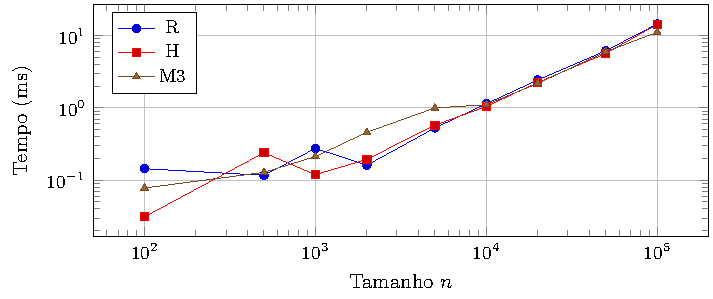
\includegraphics[width=.83\textwidth]{graficos/aleatorio_tempo.pdf}
\caption{Tempo médio por tamanho — dados aleatórios}
\label{graf:aleatorio:tempo}
\par\smallskip\footnotesize Fonte: arrays\_testados/resultados.csv. Eixos logarítmicos.
\end{grafico}
\begin{table}[htbp]
\centering\small
\caption{Comparações médias — dados aleatórios (R, H e M3)}
\label{tab:aleatorio:comparacoes}
\begin{tabular}{r r r r}
\hline
$n$ & R & H & M3 \\
\hline
100 & 595 & 636 & 640 \\
500 & 4.690 & 4.940 & 4.579 \\
1.000 & 10.481 & 10.972 & 10.373 \\
2.000 & 24.672 & 25.389 & 22.929 \\
5.000 & 70.861 & 73.162 & 65.611 \\
10.000 & 156.852 & 161.474 & 141.037 \\
20.000 & 338.200 & 347.730 & 303.752 \\
50.000 & 924.915 & 947.781 & 834.841 \\
100.000 & 1.943.232 & 1.988.771 & 1.799.683 \\
\hline
\end{tabular}
\par\smallskip\footnotesize Fonte: arrays\_testados/resultados.csv; contagens médias de operações. H e M3 usam $M=15$.
\end{table}
\begin{grafico}[H]
\centering
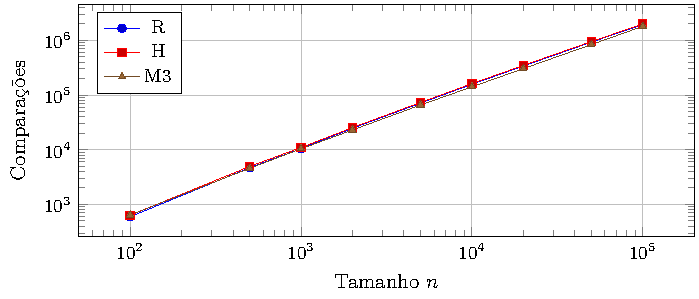
\includegraphics[width=.83\textwidth]{graficos/aleatorio_comparacoes.pdf}
\caption{Comparações médias por tamanho — dados aleatórios}
\label{graf:aleatorio:comparacoes}
\par\smallskip\footnotesize Fonte: arrays\_testados/resultados.csv. Eixos logarítmicos.
\end{grafico}
\begin{table}[htbp]
\centering\small
\caption{Trocas/movimentos médios — dados aleatórios (R, H e M3)}
\label{tab:aleatorio:movimentos}
\begin{tabular}{r r r r}
\hline
$n$ & R & H & M3 \\
\hline
100 & 244 & 416 & 414 \\
500 & 1.904 & 2.764 & 3.037 \\
1.000 & 5.473 & 7.091 & 6.913 \\
2.000 & 11.016 & 14.163 & 13.199 \\
5.000 & 32.696 & 41.103 & 36.987 \\
10.000 & 78.558 & 94.932 & 80.757 \\
20.000 & 152.928 & 186.977 & 175.539 \\
50.000 & 429.238 & 512.177 & 467.162 \\
100.000 & 883.375 & 1.049.788 & 1.003.896 \\
\hline
\end{tabular}
\par\smallskip\footnotesize Fonte: arrays\_testados/resultados.csv; contagens médias de operações. H e M3 usam $M=15$.
\end{table}
\begin{grafico}[H]
\centering
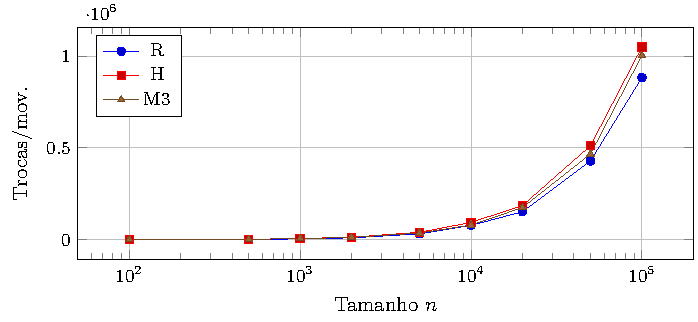
\includegraphics[width=.83\textwidth]{graficos/aleatorio_movimentos.pdf}
\caption{Trocas/movimentos médios por tamanho — dados aleatórios}
\label{graf:aleatorio:movimentos}
\par\smallskip\footnotesize Fonte: arrays\_testados/resultados.csv. Eixo horizontal logarítmico; zero preservado.
\end{grafico}
\subsection*{Interpretação: entrada aleatória}
As contagens crescem de milhares a milhões de comparações à medida que $n$ aumenta, sem a explosão quadrática determinística das entradas crescentes. Em $n=10.000$, R faz 156.852 comparações, H 161.474 e M3 141.037: a mediana reduz inspeções, mas H tem o menor tempo observado (1,04510 ms). Em $n=100.000$, M3 passa a ter menor tempo (11,11544 ms); H registra o maior número de trocas/movimentos (1.049.788 contra 883.375 de R). Isso é coerente com deslocamentos locais na inserção, não com trocas literais adicionais entre pares de posições. A não monotonicidade de tempos em alguns tamanhos (R passa de 0,27558 ms em 1.000 para 0,16082 ms em 2.000) recomenda não atribuir significado a diferenças pequenas sem dispersão e medições adicionais.

\section{Entrada crescente}
\label{sec:ordenado}
Apresentam-se as 6 dimensões registradas para dados crescentes. R indica o recursivo, H o híbrido com pivô final e M3 o híbrido com mediana-de-três.
\begin{table}[htbp]
\centering\small
\caption{Tempo médio (ms) — entrada crescente (R, H e M3)}
\label{tab:ordenado:tempo}
\begin{tabular}{r r r r}
\hline
$n$ & R & H & M3 \\
\hline
100 & 0,01412 & 0,01708 & 0,00196 \\
500 & 0,32652 & 0,36616 & 0,01086 \\
1.000 & 1,21644 & 1,21218 & 0,02226 \\
2.000 & 4,68986 & 5,43040 & 0,15874 \\
5.000 & 22,59508 & 23,17818 & 0,12780 \\
10.000 & 93,18666 & 83,49934 & 0,23122 \\
\hline
\end{tabular}
\par\smallskip\footnotesize Fonte: arrays\_testados/resultados.csv; tempos convertidos de ns para ms. H e M3 usam $M=15$.
\end{table}
\begin{grafico}[H]
\centering
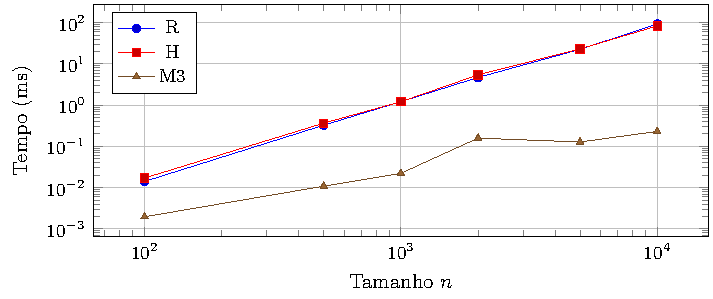
\includegraphics[width=.83\textwidth]{graficos/ordenado_tempo.pdf}
\caption{Tempo médio por tamanho — entrada crescente}
\label{graf:ordenado:tempo}
\par\smallskip\footnotesize Fonte: arrays\_testados/resultados.csv. Eixos logarítmicos.
\end{grafico}
\begin{table}[htbp]
\centering\small
\caption{Comparações médias — entrada crescente (R, H e M3)}
\label{tab:ordenado:comparacoes}
\begin{tabular}{r r r r}
\hline
$n$ & R & H & M3 \\
\hline
100 & 4.950 & 4.872 & 395 \\
500 & 124.750 & 124.672 & 3.288 \\
1.000 & 499.500 & 499.422 & 7.557 \\
2.000 & 1.999.000 & 1.998.922 & 17.094 \\
5.000 & 12.497.500 & 12.497.422 & 49.497 \\
10.000 & 49.995.000 & 49.994.922 & 108.986 \\
\hline
\end{tabular}
\par\smallskip\footnotesize Fonte: arrays\_testados/resultados.csv; contagens médias de operações. H e M3 usam $M=15$.
\end{table}
\begin{grafico}[H]
\centering
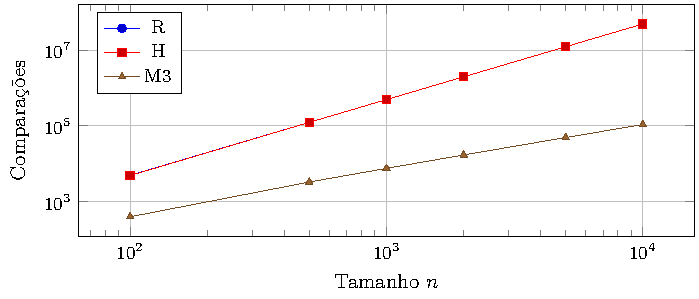
\includegraphics[width=.83\textwidth]{graficos/ordenado_comparacoes.pdf}
\caption{Comparações médias por tamanho — entrada crescente}
\label{graf:ordenado:comparacoes}
\par\smallskip\footnotesize Fonte: arrays\_testados/resultados.csv. Eixos logarítmicos.
\end{grafico}
\begin{table}[htbp]
\centering\small
\caption{Trocas/movimentos médios — entrada crescente (R, H e M3)}
\label{tab:ordenado:movimentos}
\begin{tabular}{r r r r}
\hline
$n$ & R & H & M3 \\
\hline
100 & 0 & 0 & 14 \\
500 & 0 & 0 & 104 \\
1.000 & 0 & 0 & 208 \\
2.000 & 0 & 0 & 416 \\
5.000 & 0 & 0 & 1.022 \\
10.000 & 0 & 0 & 2.046 \\
\hline
\end{tabular}
\par\smallskip\footnotesize Fonte: arrays\_testados/resultados.csv; contagens médias de operações. H e M3 usam $M=15$.
\end{table}
\begin{grafico}[H]
\centering
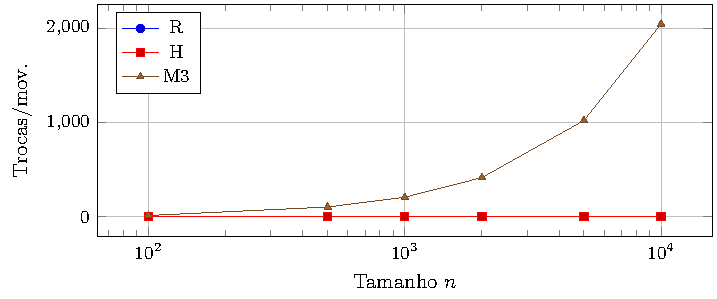
\includegraphics[width=.83\textwidth]{graficos/ordenado_movimentos.pdf}
\caption{Trocas/movimentos médios por tamanho — entrada crescente}
\label{graf:ordenado:movimentos}
\par\smallskip\footnotesize Fonte: arrays\_testados/resultados.csv. Eixo horizontal logarítmico; zero preservado.
\end{grafico}
\subsection*{Interpretação: entrada crescente}
No pivô final, cada varredura encontra o máximo da região; por isso R faz exatamente $n(n-1)/2$ comparações e nenhuma troca entre índices distintos. H elimina só 78 comparações em 10.000 valores, apesar do limiar de inserção, pois os subvetores grandes continuam degenerados. M3 escolhe inicialmente um valor central, reduzindo a profundidade efetiva nesta entrada; faz 108.986 comparações e 2.046 trocas/movimentos em 10.000 valores, contra 49.995.000 e zero de R. O resultado não significa que fazer mais trocas seja intrinsecamente melhor: o benefício decorre sobretudo de evitar milhões de inspeções nas partições desbalanceadas. A mediana não dá garantia de $O(n\log n)$ para entradas arbitrárias.

\section{Entrada decrescente}
\label{sec:inverso}
Apresentam-se as 6 dimensões registradas para dados decrescentes. R indica o recursivo, H o híbrido com pivô final e M3 o híbrido com mediana-de-três.
\begin{table}[htbp]
\centering\small
\caption{Tempo médio (ms) — entrada decrescente (R, H e M3)}
\label{tab:inverso:tempo}
\begin{tabular}{r r r r}
\hline
$n$ & R & H & M3 \\
\hline
100 & 0,00960 & 0,00758 & 0,00466 \\
500 & 0,12458 & 0,17294 & 0,01130 \\
1.000 & 0,52140 & 0,63826 & 0,02494 \\
2.000 & 2,03772 & 2,82486 & 0,06720 \\
5.000 & 14,27006 & 17,92168 & 0,15448 \\
10.000 & 60,29422 & 65,13762 & 0,61380 \\
\hline
\end{tabular}
\par\smallskip\footnotesize Fonte: arrays\_testados/resultados.csv; tempos convertidos de ns para ms. H e M3 usam $M=15$.
\end{table}
\begin{grafico}[H]
\centering
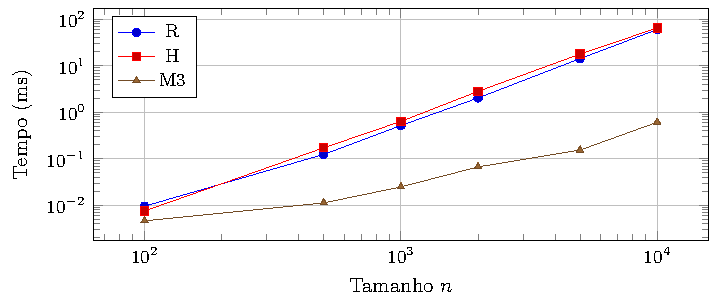
\includegraphics[width=.83\textwidth]{graficos/inverso_tempo.pdf}
\caption{Tempo médio por tamanho — entrada decrescente}
\label{graf:inverso:tempo}
\par\smallskip\footnotesize Fonte: arrays\_testados/resultados.csv. Eixos logarítmicos.
\end{grafico}
\begin{table}[htbp]
\centering\small
\caption{Comparações médias — entrada decrescente (R, H e M3)}
\label{tab:inverso:comparacoes}
\begin{tabular}{r r r r}
\hline
$n$ & R & H & M3 \\
\hline
100 & 4.950 & 4.950 & 878 \\
500 & 124.750 & 124.750 & 7.281 \\
1.000 & 499.500 & 499.500 & 16.783 \\
2.000 & 1.999.000 & 1.999.000 & 38.105 \\
5.000 & 12.497.500 & 12.497.500 & 109.138 \\
10.000 & 49.995.000 & 49.995.000 & 240.720 \\
\hline
\end{tabular}
\par\smallskip\footnotesize Fonte: arrays\_testados/resultados.csv; contagens médias de operações. H e M3 usam $M=15$.
\end{table}
\begin{grafico}[H]
\centering
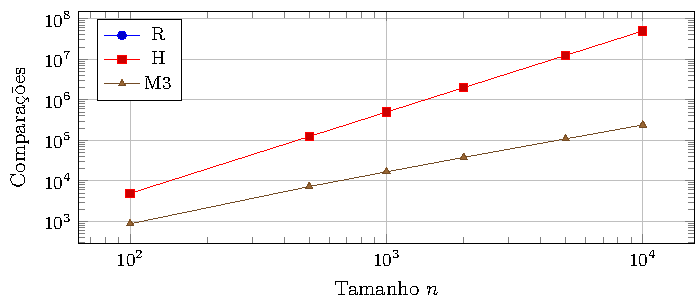
\includegraphics[width=.83\textwidth]{graficos/inverso_comparacoes.pdf}
\caption{Comparações médias por tamanho — entrada decrescente}
\label{graf:inverso:comparacoes}
\par\smallskip\footnotesize Fonte: arrays\_testados/resultados.csv. Eixos logarítmicos.
\end{grafico}
\begin{table}[htbp]
\centering\small
\caption{Trocas/movimentos médios — entrada decrescente (R, H e M3)}
\label{tab:inverso:movimentos}
\begin{tabular}{r r r r}
\hline
$n$ & R & H & M3 \\
\hline
100 & 50 & 147 & 567 \\
500 & 250 & 347 & 4.398 \\
1.000 & 500 & 597 & 9.622 \\
2.000 & 1.000 & 1.097 & 21.021 \\
5.000 & 2.500 & 2.597 & 55.627 \\
10.000 & 5.000 & 5.097 & 119.730 \\
\hline
\end{tabular}
\par\smallskip\footnotesize Fonte: arrays\_testados/resultados.csv; contagens médias de operações. H e M3 usam $M=15$.
\end{table}
\begin{grafico}[H]
\centering
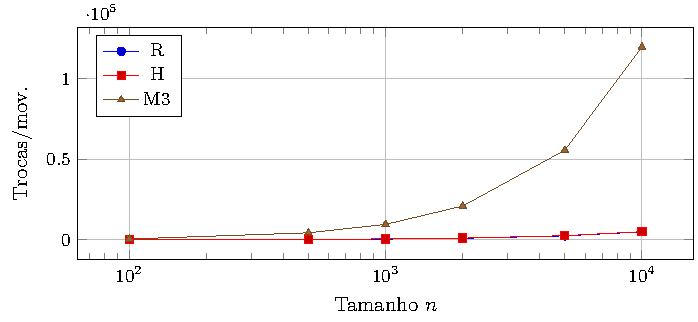
\includegraphics[width=.83\textwidth]{graficos/inverso_movimentos.pdf}
\caption{Trocas/movimentos médios por tamanho — entrada decrescente}
\label{graf:inverso:movimentos}
\par\smallskip\footnotesize Fonte: arrays\_testados/resultados.csv. Eixo horizontal logarítmico; zero preservado.
\end{grafico}
\subsection*{Interpretação: entrada decrescente}
O primeiro pivô final é mínimo, e os próximos pivôs permanecem extremos após as partições, levando novamente a $n(n-1)/2$ comparações em R. Diferentemente da entrada crescente, a posição final do pivô frequentemente difere de seu índice original: R registra 5.000 trocas em 10.000 valores; H registra 5.097 movimentos/trocas. M3 diminui as comparações para 240.720 e o tempo para 0,61380 ms, mas contabiliza 119.730 movimentações. A reorganização adicional é necessária para formar partições menos desiguais nesta implementação; tempo e número de movimentos não precisam variar na mesma proporção.

\section{Muitos valores repetidos}
\label{sec:duplicados}
Apresentam-se as 9 dimensões registradas para dados com duplicatas. R indica o recursivo, H o híbrido com pivô final e M3 o híbrido com mediana-de-três.
\begin{table}[htbp]
\centering\small
\caption{Tempo médio (ms) — muitos valores repetidos (R, H e M3)}
\label{tab:duplicados:tempo}
\begin{tabular}{r r r r}
\hline
$n$ & R & H & M3 \\
\hline
100 & 0,00206 & 0,00202 & 0,00228 \\
500 & 0,03054 & 0,00902 & 0,00784 \\
1.000 & 0,03646 & 0,03470 & 0,03760 \\
2.000 & 0,18880 & 0,07838 & 0,07304 \\
5.000 & 0,43580 & 0,25796 & 0,23756 \\
10.000 & 0,82768 & 0,71022 & 0,58158 \\
20.000 & 1,56256 & 1,36438 & 1,15740 \\
50.000 & 5,14288 & 4,38076 & 3,76142 \\
100.000 & 8,97956 & 8,04022 & 8,11022 \\
\hline
\end{tabular}
\par\smallskip\footnotesize Fonte: arrays\_testados/resultados.csv; tempos convertidos de ns para ms. H e M3 usam $M=15$.
\end{table}
\begin{grafico}[H]
\centering
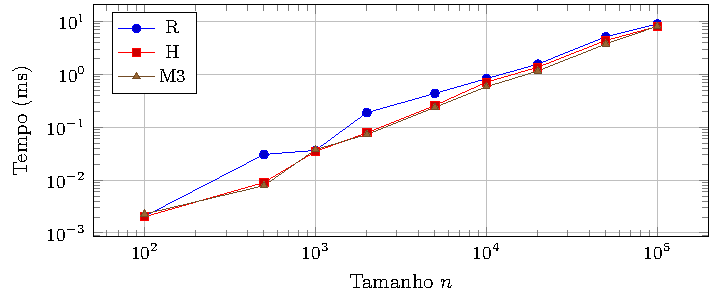
\includegraphics[width=.83\textwidth]{graficos/duplicados_tempo.pdf}
\caption{Tempo médio por tamanho — muitos valores repetidos}
\label{graf:duplicados:tempo}
\par\smallskip\footnotesize Fonte: arrays\_testados/resultados.csv. Eixos logarítmicos.
\end{grafico}
\begin{table}[htbp]
\centering\small
\caption{Comparações médias — muitos valores repetidos (R, H e M3)}
\label{tab:duplicados:comparacoes}
\begin{tabular}{r r r r}
\hline
$n$ & R & H & M3 \\
\hline
100 & 749 & 456 & 493 \\
500 & 5.768 & 4.372 & 3.883 \\
1.000 & 14.135 & 11.363 & 10.182 \\
2.000 & 30.732 & 25.016 & 21.355 \\
5.000 & 83.425 & 69.296 & 65.824 \\
10.000 & 167.611 & 139.666 & 144.327 \\
20.000 & 376.521 & 320.318 & 296.273 \\
50.000 & 1.008.325 & 867.115 & 776.512 \\
100.000 & 2.240.874 & 1.960.416 & 1.706.146 \\
\hline
\end{tabular}
\par\smallskip\footnotesize Fonte: arrays\_testados/resultados.csv; contagens médias de operações. H e M3 usam $M=15$.
\end{table}
\begin{grafico}[H]
\centering
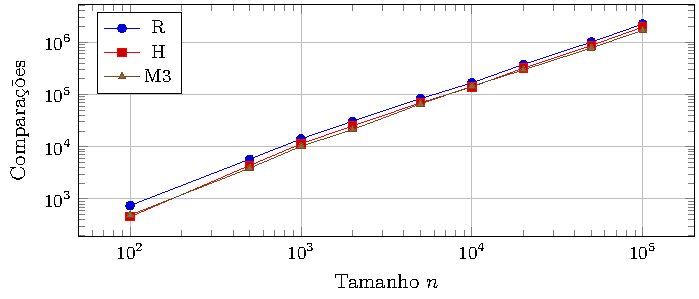
\includegraphics[width=.83\textwidth]{graficos/duplicados_comparacoes.pdf}
\caption{Comparações médias por tamanho — muitos valores repetidos}
\label{graf:duplicados:comparacoes}
\par\smallskip\footnotesize Fonte: arrays\_testados/resultados.csv. Eixos logarítmicos.
\end{grafico}
\begin{table}[htbp]
\centering\small
\caption{Trocas/movimentos médios — muitos valores repetidos (R, H e M3)}
\label{tab:duplicados:movimentos}
\begin{tabular}{r r r r}
\hline
$n$ & R & H & M3 \\
\hline
100 & 175 & 175 & 172 \\
500 & 1.835 & 1.961 & 2.092 \\
1.000 & 6.033 & 6.164 & 4.999 \\
2.000 & 8.928 & 9.131 & 8.893 \\
5.000 & 27.640 & 28.579 & 30.992 \\
10.000 & 60.102 & 62.072 & 61.848 \\
20.000 & 152.134 & 156.037 & 142.461 \\
50.000 & 367.209 & 375.556 & 340.456 \\
100.000 & 884.921 & 903.629 & 829.248 \\
\hline
\end{tabular}
\par\smallskip\footnotesize Fonte: arrays\_testados/resultados.csv; contagens médias de operações. H e M3 usam $M=15$.
\end{table}
\begin{grafico}[H]
\centering
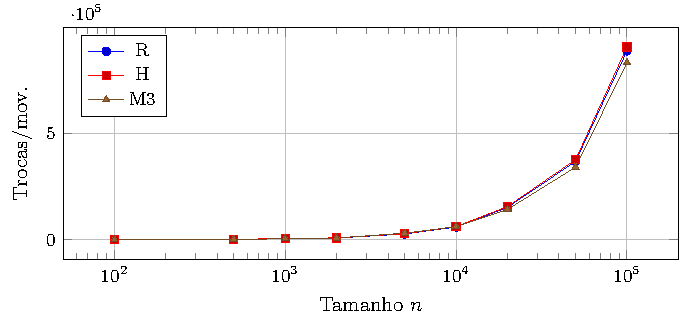
\includegraphics[width=.83\textwidth]{graficos/duplicados_movimentos.pdf}
\caption{Trocas/movimentos médios por tamanho — muitos valores repetidos}
\label{graf:duplicados:movimentos}
\par\smallskip\footnotesize Fonte: arrays\_testados/resultados.csv. Eixo horizontal logarítmico; zero preservado.
\end{grafico}
\subsection*{Interpretação: muitos valores repetidos}
Em 10.000 valores repetidos, M3 registra 0,58158 ms, abaixo de R (0,82768 ms) e H (0,71022 ms), embora H faça menos comparações que M3 (139.666 contra 144.327). Em 100.000, H supera M3 por apenas 0,07000 ms, sem que os dados disponíveis permitam declarar uma diferença confiável. O operador $\leq$ da partição coloca iguais à esquerda; a mediana entre três candidatos não separa uma região central de iguais. A quantidade de chaves possíveis cresce com $n$, portanto este ensaio não demonstra que todos os iguais seriam processados em $O(n\log n)$; uma partição em três vias seria uma extensão apropriada.

\section{Pior caso explícito}
\label{sec:pior}
Apresentam-se as 7 dimensões registradas para dados do pior caso explícito. R indica o recursivo, H o híbrido com pivô final e M3 o híbrido com mediana-de-três.
\begin{table}[htbp]
\centering\small
\caption{Tempo médio (ms) — pior caso explícito (R, H e M3)}
\label{tab:pior:tempo}
\begin{tabular}{r r r r}
\hline
$n$ & R & H & M3 \\
\hline
100 & 0,01050 & 0,00820 & 0,00128 \\
200 & 0,02352 & 0,03092 & 0,00240 \\
500 & 0,14554 & 0,28136 & 0,01004 \\
1.000 & 0,56778 & 0,77766 & 0,01532 \\
2.000 & 2,42954 & 3,53726 & 0,03578 \\
5.000 & 16,92574 & 25,46218 & 0,11224 \\
10.000 & 68,96428 & 82,97444 & 0,23330 \\
\hline
\end{tabular}
\par\smallskip\footnotesize Fonte: arrays\_testados/resultados.csv; tempos convertidos de ns para ms. H e M3 usam $M=15$.
\end{table}
\begin{grafico}[H]
\centering
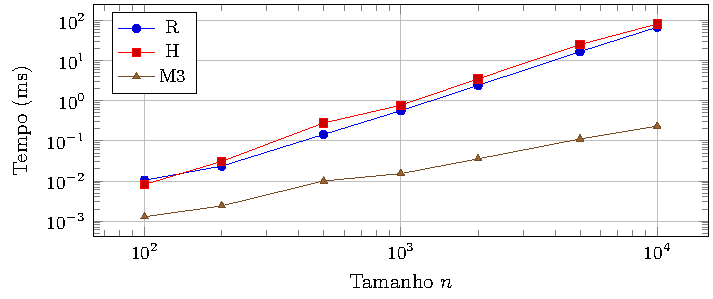
\includegraphics[width=.83\textwidth]{graficos/pior_tempo.pdf}
\caption{Tempo médio por tamanho — pior caso explícito}
\label{graf:pior:tempo}
\par\smallskip\footnotesize Fonte: arrays\_testados/resultados.csv. Eixos logarítmicos.
\end{grafico}
\begin{table}[htbp]
\centering\small
\caption{Comparações médias — pior caso explícito (R, H e M3)}
\label{tab:pior:comparacoes}
\begin{tabular}{r r r r}
\hline
$n$ & R & H & M3 \\
\hline
100 & 4.950 & 4.872 & 395 \\
200 & 19.900 & 19.822 & 988 \\
500 & 124.750 & 124.672 & 3.288 \\
1.000 & 499.500 & 499.422 & 7.557 \\
2.000 & 1.999.000 & 1.998.922 & 17.094 \\
5.000 & 12.497.500 & 12.497.422 & 49.497 \\
10.000 & 49.995.000 & 49.994.922 & 108.986 \\
\hline
\end{tabular}
\par\smallskip\footnotesize Fonte: arrays\_testados/resultados.csv; contagens médias de operações. H e M3 usam $M=15$.
\end{table}
\begin{grafico}[H]
\centering
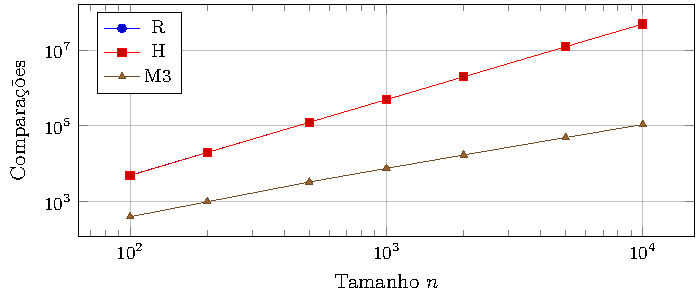
\includegraphics[width=.83\textwidth]{graficos/pior_comparacoes.pdf}
\caption{Comparações médias por tamanho — pior caso explícito}
\label{graf:pior:comparacoes}
\par\smallskip\footnotesize Fonte: arrays\_testados/resultados.csv. Eixos logarítmicos.
\end{grafico}
\begin{table}[htbp]
\centering\small
\caption{Trocas/movimentos médios — pior caso explícito (R, H e M3)}
\label{tab:pior:movimentos}
\begin{tabular}{r r r r}
\hline
$n$ & R & H & M3 \\
\hline
100 & 0 & 0 & 14 \\
200 & 0 & 0 & 30 \\
500 & 0 & 0 & 104 \\
1.000 & 0 & 0 & 208 \\
2.000 & 0 & 0 & 416 \\
5.000 & 0 & 0 & 1.022 \\
10.000 & 0 & 0 & 2.046 \\
\hline
\end{tabular}
\par\smallskip\footnotesize Fonte: arrays\_testados/resultados.csv; contagens médias de operações. H e M3 usam $M=15$.
\end{table}
\begin{grafico}[H]
\centering
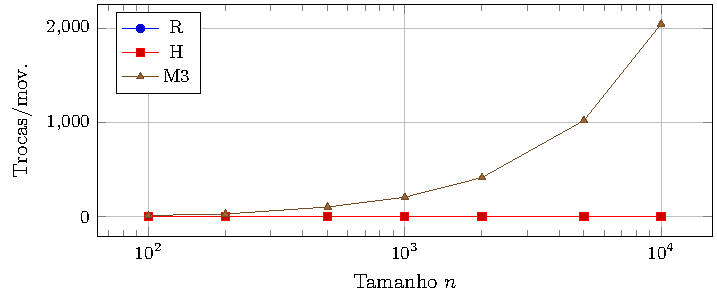
\includegraphics[width=.83\textwidth]{graficos/pior_movimentos.pdf}
\caption{Trocas/movimentos médios por tamanho — pior caso explícito}
\label{graf:pior:movimentos}
\par\smallskip\footnotesize Fonte: arrays\_testados/resultados.csv. Eixo horizontal logarítmico; zero preservado.
\end{grafico}
\subsection*{Interpretação: pior caso explícito com pivô final}
Esta massa é crescente e distinta, como a seção anterior de ordenado, mas foi executada novamente para identificar expressamente o caso adverso de R e H. Em $n=1.000$, R faz 499.500 comparações; em $n=10.000$, 49.995.000: aumentar a entrada dez vezes aumenta as comparações cerca de cem vezes. H faz 49.994.922 comparações em 10.000. M3 faz 108.986 nessa entrada e mantém tempo inferior a 1 ms em todos os tamanhos ensaiados. \emph{Pior caso explícito} designa aqui o pior caso da seleção de pivô final, não um pior caso construído contra M3. As zero trocas de R e H no vetor crescente refletem a convenção de ignorar troca de um índice por ele mesmo; não significam ausência de custo.



\section{Síntese quantitativa e limites da comparação}

A Tabela~\ref{tab:panorama10000} põe as três versões lado a lado sob o mesmo tamanho, para facilitar a leitura transversal entre as seções detalhadas. O cenário adverso crescente foi executado separadamente e aparece novamente na última linha; valores iguais de contadores entre essas duas linhas são esperados, mas tempos iguais não são exigidos.

\begin{table}[htbp]
\centering
\caption{Panorama dos tempos médios para $n=10.000$ (ms; menor valor observado em negrito)}
\label{tab:panorama10000}
\begin{tabular}{l r r r}
\hline
Cenário & R & H & M3 \\
\hline
Aleatório & 1,14024 & \textbf{1,04510} & 1,10436 \\
Crescente & 93,18666 & 83,49934 & \textbf{0,23122} \\
Decrescente & 60,29422 & 65,13762 & \textbf{0,61380} \\
Muitos duplicados & 0,82768 & 0,71022 & \textbf{0,58158} \\
Pior caso (crescente) & 68,96428 & 82,97444 & \textbf{0,23330} \\
\hline
\end{tabular}
\par\smallskip\footnotesize Fonte: \path{arrays_testados/resultados.csv}; menor tempo apenas nesta execução.\normalsize
\end{table}

As diferenças de escala são mais informativas do que a simples posição de primeiro lugar: na crescente de 10.000 elementos, R levou aproximadamente 403 vezes o tempo de M3, enquanto em aleatório o menor tempo observado de H supera o de M3 por apenas cerca de 0,059 ms. Não se deve atribuir certeza à última diferença sem medições de dispersão. No inverso, o bom tempo de M3 convive com 119.730 trocas/movimentos contra 5.000 de R: contar movimentações isoladamente não é suficiente para predizer duração. O ensaio com duplicatas mostra que essa vantagem também não decorre de uma solução completa para valores iguais; a partição permanece de duas vias.

No tamanho de 10.000, a mediana-de-três reduz as comparações em dados crescentes de 49.995.000 (R) para 108.986 (M3), fator de aproximadamente 459. Em dados inversos, a redução é para 240.720, fator de aproximadamente 208, embora M3 faça mais movimentações. O híbrido de pivô final permanece quadrático nessas duas entradas; o corte em $M=15$ altera apenas as partições finais. No pior caso explícito de 10.000, R faz 49.995.000 comparações, H faz 49.994.922 e M3 faz 108.986; a identidade entre este caso e a massa crescente explica as contagens iguais, enquanto os tempos distintos são medições realizadas em momentos diferentes.

Em 100.000 valores aleatórios, M3 tem 11,11544 ms, aproximadamente 23\% menos que R (14,45802 ms), mas em 50.000 o menor tempo é de H (5,65368 ms, contra 5,96680 ms de M3). Em 100.000 valores repetidos, M3 contabiliza menos comparações que H (1.706.146 contra 1.960.416), mas leva 8,11022 ms contra 8,04022 ms. Essas inversões são compatíveis com diferenças entre métricas e variação temporal. A ausência de desvio padrão, intervalo de confiança e controle da carga do sistema impede alegar significância estatística. Finalmente, a massa de repetidos tem até $n/10$ chaves possíveis: não equivale ao vetor de chaves todas iguais, que poderia degenerar a partição de duas vias nas três versões.

\chapter{Conclusão}
\label{cap:conclusao}

\section{Síntese dos resultados}

Foram examinadas três implementações de Quicksort sobre cinco cenários e 37 combinações de tipo/tamanho, com três aquecimentos e cinco medições por versão, perfazendo 111 médias registradas. A calibração isolada do híbrido de pivô final escolheu $M=15$ entre dez candidatos; o mesmo limiar foi empregado na versão com mediana-de-três. A instrumentação permite relacionar o tempo às comparações e às trocas/movimentos, desde que as movimentações de Insertion Sort não sejam confundidas com trocas de pares de índices.

As entradas crescentes e decrescentes expuseram o custo quadrático das versões com pivô final: para $n=10.000$, ambas realizaram aproximadamente 50 milhões de comparações. A hibridização isolada praticamente não alterou essa contagem no vetor crescente; pela condição $n<M$, reduziu-a em apenas 78 unidades. A mediana-de-três reduziu as comparações a 108.986 nesse vetor e a 240.720 no inverso, mostrando a vantagem de evitar os pivôs extremos dessas entradas específicas. Os contadores do caso crescente repetido como \emph{pior caso explícito} coincidem com o primeiro, confirmando que é uma repetição controlada, não uma construção adversa diferente.

\section{Conclusões e possibilidades de extensão}

Em dados aleatórios e repetidos, a vantagem em tempo não foi uniforme. M3 foi a opção mais rápida entre as três em 100.000 valores aleatórios, porém H venceu M3 em 50.000 aleatórios e por pequena margem em 100.000 repetidos. Portanto, \textbf{não há um algoritmo mais rápido em todas as entradas medidas}; nem a mediana-de-três elimina o pior caso teórico quando a partição em duas vias encontra chaves iguais. O valor $M=15$ descreve o menor tempo de uma calibração específica, não uma constante universal.

Em termos práticos, o estudo sustenta usar a mediana-de-três quando se deseja reduzir a sensibilidade desta implementação às entradas crescentes e decrescentes examinadas; não sustenta afirmar que ela elimina os piores casos nem que o corte por inserção, sozinho, corrige um pivô adverso. O benefício do híbrido depende da relação entre o custo das partições evitadas e o custo da inserção local. Por isso, a escolha do limiar deve ser relatada com a massa e o procedimento que a produziram, e diferenças temporais pequenas devem ser interpretadas como observações, não como garantias para outra máquina.

O número reduzido de medições, a ausência de variância, as diferenças de massa conforme $n$ e a falta de controle das condições de carga restringem as conclusões temporais a esta execução. Como trabalhos futuros, recomendam-se repetições com múltiplas sementes, estatísticas de dispersão, randomização da ordem de medição e avaliação de partição ternária para duplicatas. Pode-se também comparar um limite de profundidade com fallback para um algoritmo de pior caso $O(n\log n)$, deixando explícito que essa técnica \emph{não} está presente no código avaliado.

% PÓS-TEXTUAIS %%
% Bibliografia no arquivo 'Dissertacao.bib'
% Alterar o título das referências para somente 'Referências'
%\renewcommand{\bibname}{Referências}
\bibliographystyle{abnt-alf}
\bibliography{Referencias}


% Para forçar que os apêndices e anexos comecem no anverso
%\setboolean{@openright}{true}

%\apendice
%\begin{apendice}
%%------------------------------------------------------------------------------------------------------------------------------------------------------
% Reiniciar numeração das figuras que aparecem no apêndice
\setcounter{figure}{0}

\chapter{Primeiro apêndice}
\label{apend:codigoMpe}

% Para diminuir espaçamento entre o título e o texto
\vspace{-1.9cm}

Textos ou documentos elaborados pelo autor, como por exemplo código-fonte.


%\end{apendice}

%\anexo
%% Nome do Anexo
\chapter{Primeiro Anexo}

% Para diminuir espa�amento entre o t�tulo e o texto
\vspace{-1.9cm}

% Texto
Textos ou documentos não elaborados pelo autor.

\end{document}
